\section{Synergistic}
The synergistic analysis in this work varied two parameters at a time to 
investigate some of the combined effects of the input parameters. Synergistic 
sensitivity analysis helps to identify if the combined effect of two parameters 
has a greater impact on the metrics that when varying a single parameter. 

\subsection{Scenario 7}\label{sec:s7_synergistic}
We ran synergistic 
analysis on all combinations of two input parameters studied in the \gls{OAT} 
analysis, except combinations of two specified build shares. The
results presented here are only a small subsection of the analysis performed, 
with the remaining results in Appendix \ref{app:s7_synergistic}.

\subsubsection{LWR lifetime and VOYGR build share}
When the percent of \glspl{LWR} operating for 80 years and the VOYGR build share 
were varied, the results are consistent with the results from varying 
each of the parameters by themselves. The effect on the \gls{HALEU} mass 
(Figure \ref{fig:lwr_voygr_share_enr_u}) is fairly uniform across the 
parameter space. As the VOYGR build share and percent of \gls{LWR} with 
extended licenses increase the \gls{HALEU} mass required decreases, 
which is consistent with the results of the \gls{OAT} analysis for these 
parameters. By combining these two parameters, there is a greater 
decrease in the \gls{HALEU} mass than the decrease observed by just varying 
a single parameter. The other \gls{HALEU} metrics, the \gls{HALEU} \gls{SWU} 
and \gls{HALEU} feed, als decrease in a similar manner as the \gls{HALEU} mass. 

\begin{figure}[ht]
    \centering
    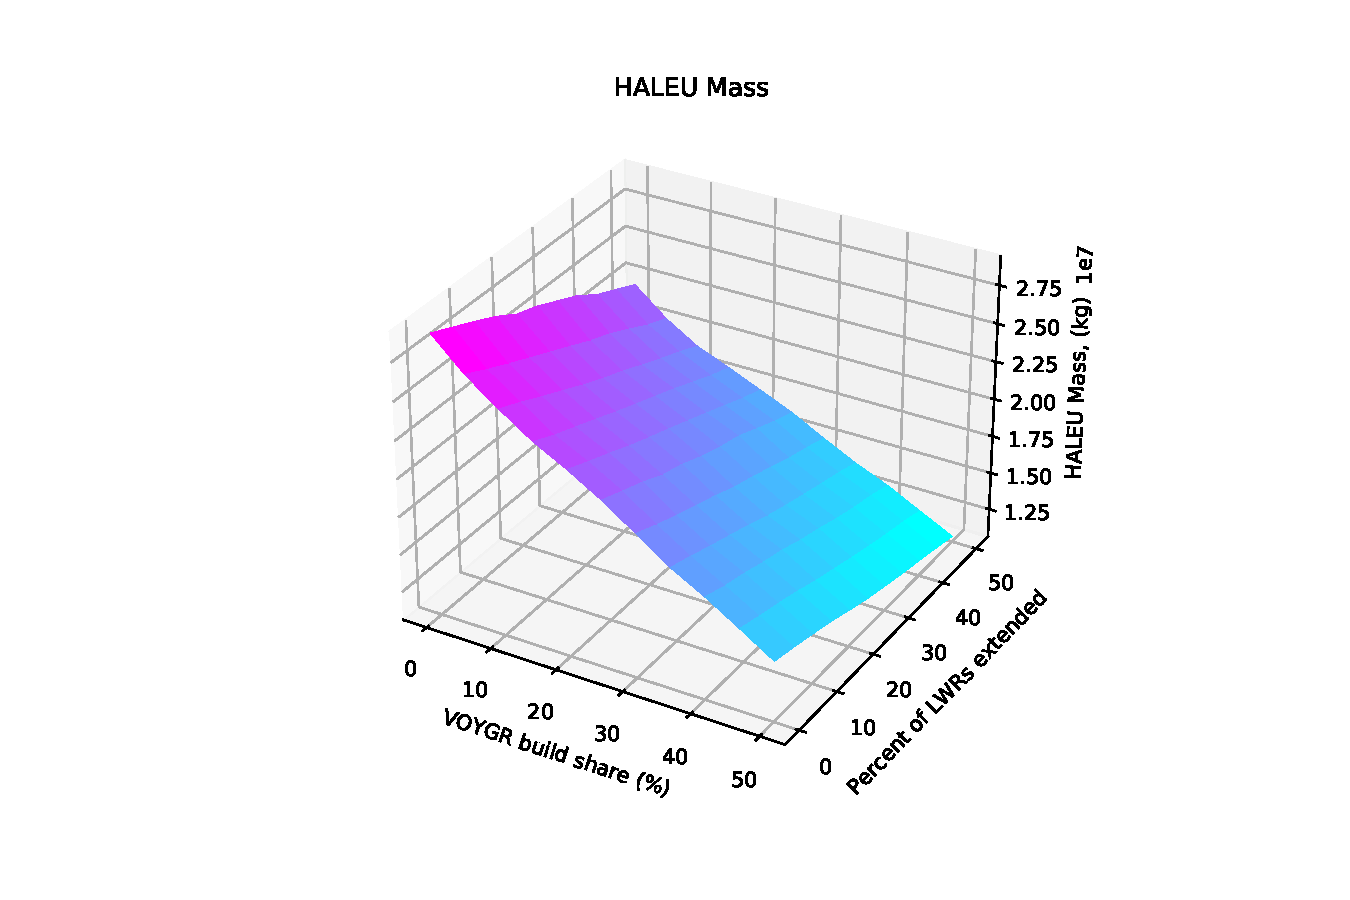
\includegraphics[scale=0.7,trim=120 0 120 30, clip]{lwr_voygr_share_haleu.pdf}
    \caption{Effect of the LWR lifetime and VOYGR build share on the HALEU mass.}
    \label{fig:lwr_voygr_share_haleu}
\end{figure}

The total enriched uranium mass decreases with increasing \gls{LWR} 
lifetimes, but increases with increasing VOYGR build share. There is a 
greater decrease in the total fuel mass required as the \gls{LWR} 
lifetime increases for greater values of VOYGR build share. 
\begin{figure}[ht]
    \centering
    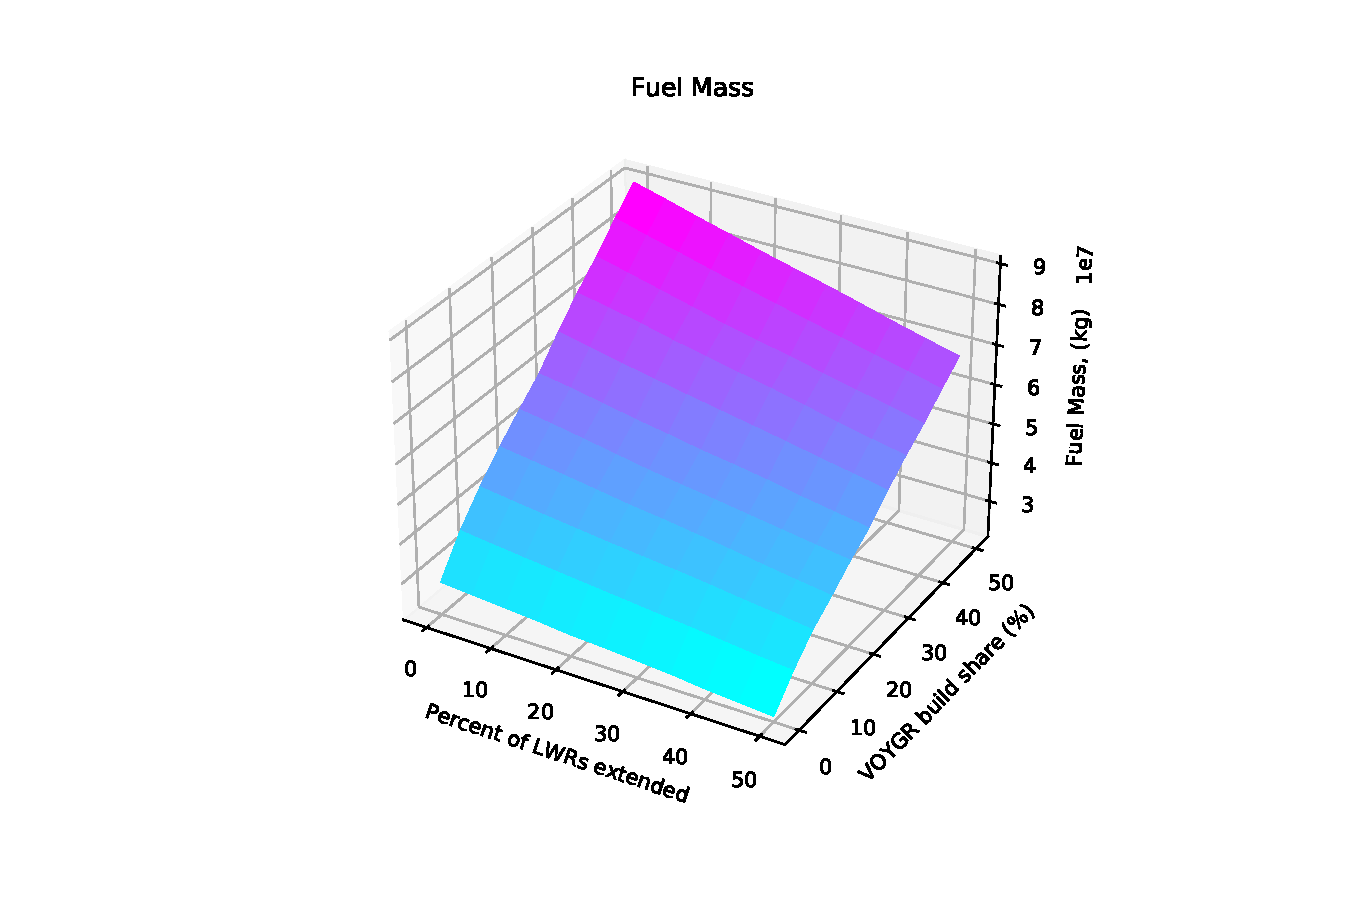
\includegraphics[scale=0.7,trim=120 0 120 30, clip]{lwr_voygr_share_enr_u.pdf}
    \caption{Effect of the LWR lifetime and VOYGR build share on 
    the total enriched uranium mass.}
    \label{fig:lwr_voygr_share_enr_u}
\end{figure}

\subsubsection{Xe-100 build share and Xe-100 burnup}
When the Xe-100 build share and discharge burnup are varied together
there is a strong combined effect on the metrics. The \gls{HALEU} 
mass required (figure \ref{fig:xe100_share_xe100_burnup_haleu}) 
increases as the burnup decreases and as the Xe-100 share increases.
The combined effect of these parameters is pronounced, such that there 
is a large increase in the \gls{HALEU} mass as the Xe-100 burnup 
reaches its minimum and the Xe-100 build share reaches its maximum. This 
results stems from a larger portion of the advanced reactor fleet 
using its fuel less efficiently as this corner of the input space is 
reached. This result suggests that the discharge burnup of an advanced 
reactor should be considered when determining the build share of a reactor
type, if this metric is important. 

\begin{figure}[h!]
    \centering
    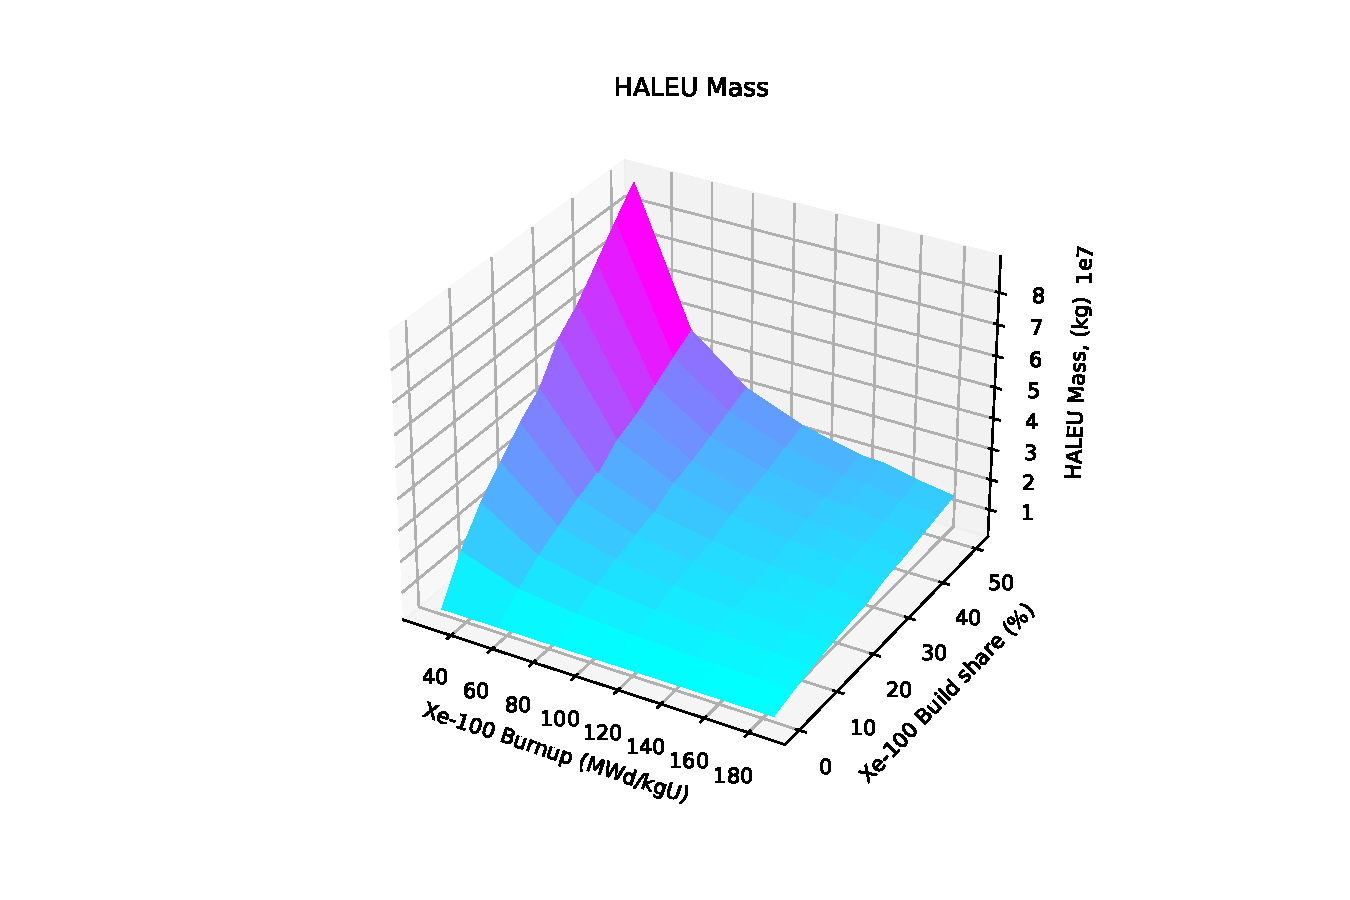
\includegraphics[scale=0.7, trim=120 0 120 30, clip]{xe100_share_xe100_burnup_haleu.pdf}
    \caption{Effect of Xe-100 discharge burnup and Xe-100 build share 
    on HALEU mass.}
    \label{fig:xe100_share_xe100_burnup_haleu}
\end{figure}

The total fuel mass reaches a minimum with a maximum Xe-100 build share 
and Xe-100 discharge burnup, which matches the trends observed in the 
\gls{OAT} analysis. A minimum is reach in this corner of the parameter 
space because more of the advanced reactor fleet is getting more 
energy out of the fuel used, so less fuel is required. Variations in the 
Xe-100 burnup do not affect the results when there is a 0\% Xe-100 build 
share because no Xe-100s are deployed. The Xe-100 build share does not 
greatly affect the fuel mass required when the Xe-100 has a discharge 
burnup of 28 MWd/kgU (the lowest value used in this work) because at this 
burnup level, the Xe-100 requires a similar amount of enriched uranium as 
the VOYGR for each 18 month period. Therefore, as the VOYGRs are replaced 
with Xe-100s as the Xe-100 build share increases the cumulative total 
fuel mass required does not change much. 

\begin{figure}[h!]
    \centering
    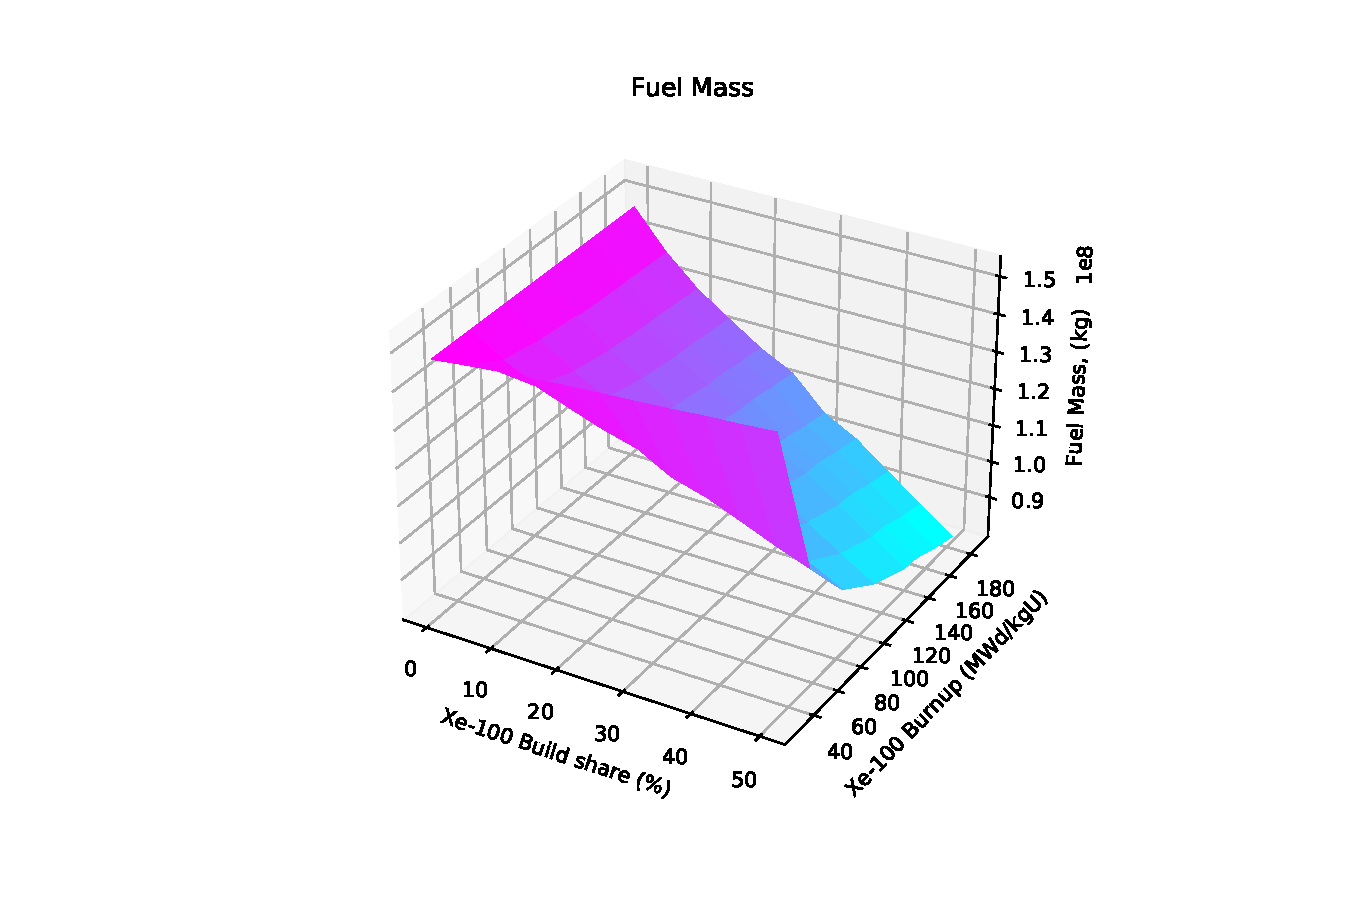
\includegraphics[scale=0.7, trim=120 0 120 30, clip]{xe100_share_xe100_burnup_enr_u.pdf}
    \caption{Effect of xe-100 discharge burnup and Xe-100 build share 
    on total fuel mass.}
    \label{fig:xe100_share_xe100_burnup_enr_u}
\end{figure}

\subsubsection{MMR build share and Xe-100 burnup}
When the \gls{MMR} build share and Xe-100 burnup are varied together, 
the effect on the metrics is not as consistent as the results from varying 
other pairs of parameters. As the Xe-100 burnup increases the fuel mass 
decreases. However, the effect of increasing the \gls{MMR} build share 
is dependent on the Xe-100 discharge burnup. At smaller Xe-100 discharge 
burnup values the fuel mass decreases with increasing \gls{MMR} build share. 
But at larger Xe-100 discharge burnup values the fuel mass increases 
with increasing \gls{MMR} build share. The different trends result from 
changes in how much fuel the Xe-100 requires at each refueling and 
the difference between that and the amount of fuel required by the \gls{MMR}.
At the lowest burnup values, the Xe-100 requires more fuel than the 
\gls{MMR}, so as more of the advanced reactor fleet is \glspl{MMR}, the 
total mass of fuel required in the transition decreases. However, as 
the Xe-100 burnup increases the Xe-100 requires less fuel than the 
\gls{MMR}. Therefore, requiring more of the advanced reactor fleet to be 
\glspl{MMR} increases the total fuel mass required by advanced reactors in 
the transition. This pattern of results is observed for all six metrics
considered in this work. 

\begin{figure}[h!]
    \centering
    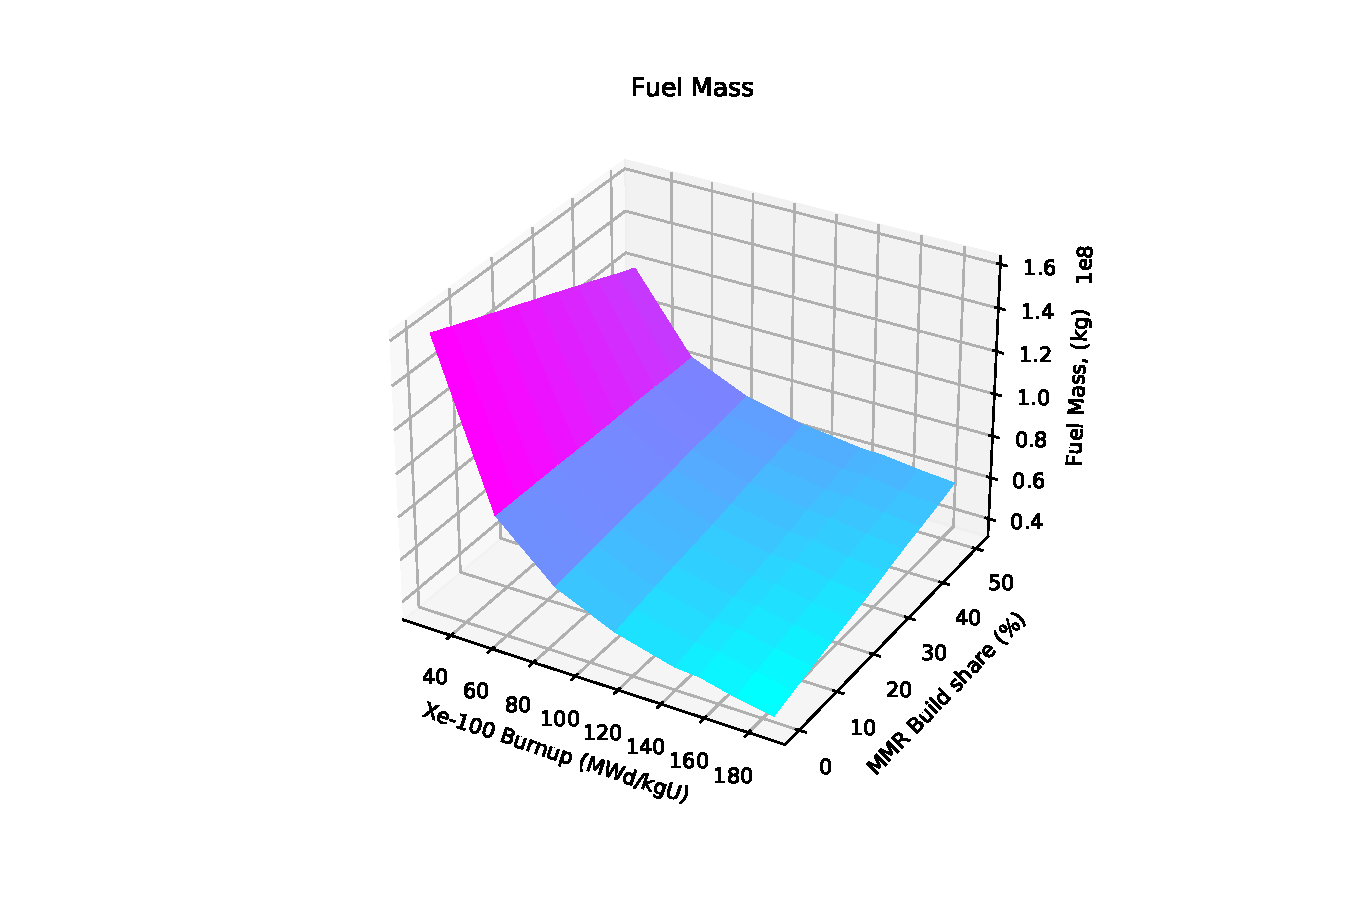
\includegraphics[scale=0.7, trim=120 0 120 30, clip]{mmr_share_xe100_burnup_enr_u.pdf}
    \caption{Effect of xe-100 discharge burnup and MMR build share 
    on total fuel mass.}
    \label{fig:mmr_share_xe100_burnup_enr_u}
\end{figure}


\subsubsection{Transition start and Xe-100 build share}
As Figure \ref{fig:ts_xe100_share_enr_u} shows, as the Xe-100 build 
share increases the total fuel mass decreases. However, there is little 
effect in the total fuel mass as the transition start time is delayed. This 
observation occurs because the magnitude of the effect on the fuel mass 
from varying the Xe-100 build share is greater than the magnitude of 
the effect from varying the transition start time. This is consistent 
with the results from the \gls{OAT} analysis, and is observed for five 
of the metrics considered in this work. This result suggests that the 
transition start time is not as important as the other parameters when 
trying to minimize or maximize certain metrics. 

\begin{figure}[h!]
    \centering
    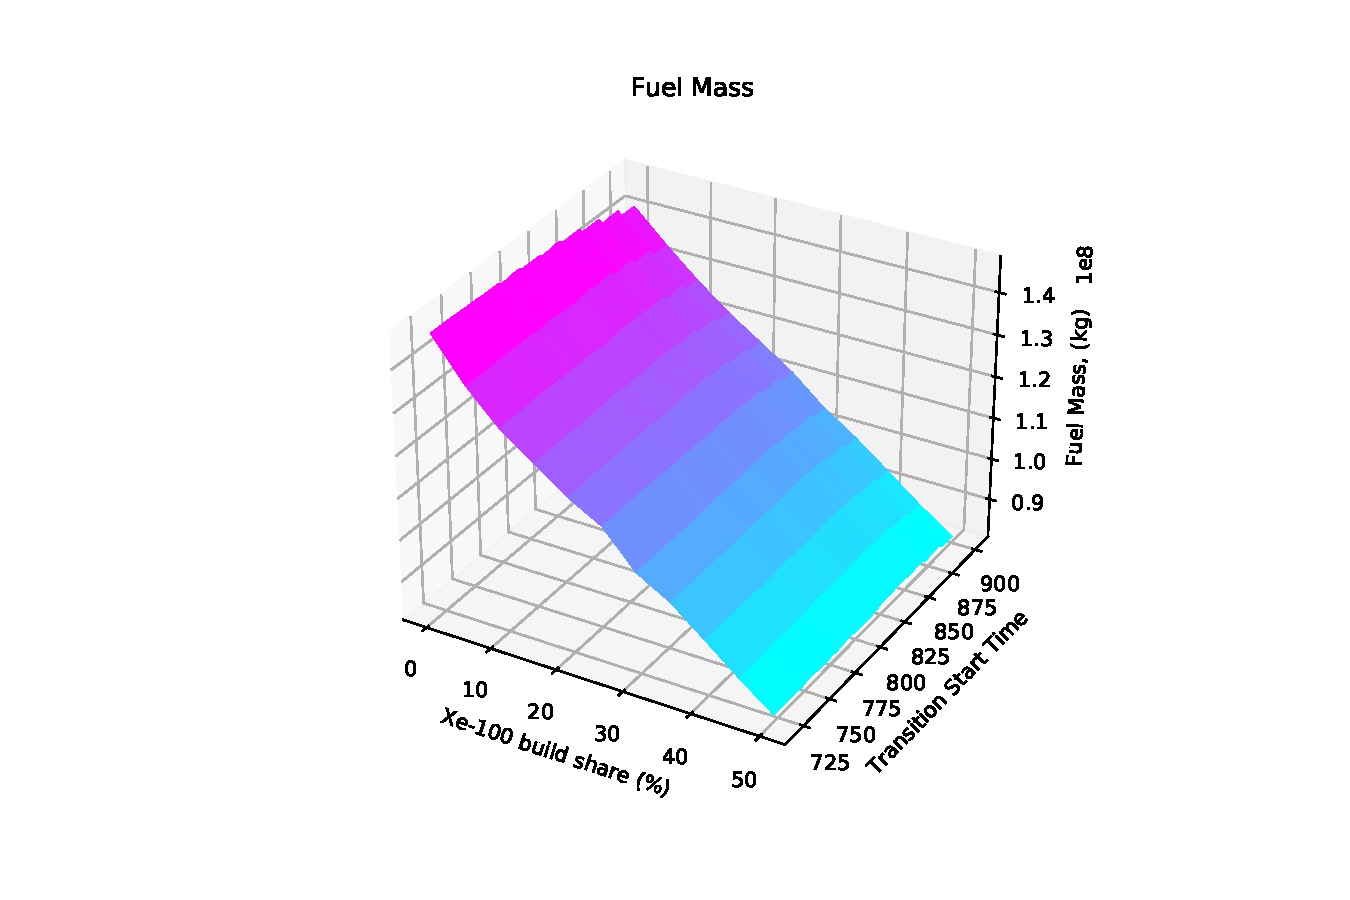
\includegraphics[scale=0.7, trim=120 0 120 0, clip]{ts_xe100_share_enr_u.pdf}
    \caption{Effect of transition start time and Xe-100 build share 
    on total fuel mass.}
    \label{fig:ts_xe100_share_enr_u}
\end{figure}

The effect of varying these two parameters is the opposite when the total 
\gls{SWU} capacity is considered: varying the transition start time has 
a greater impact on the metric than varying the Xe-100 build share. This 
result stems from the similar \gls{SWU} capacities needed for the Xe-100 
and VOYGR leading to little change in the total \gls{SWU} capacity when 
varying the Xe-100 build share. Therefore, the transition start time has 
more impact on this metric than the Xe-100 build share, and there is little 
of a combined effect observed because of the small impact from each parameter 
on this metric. 

\begin{figure}[h!]
    \centering
    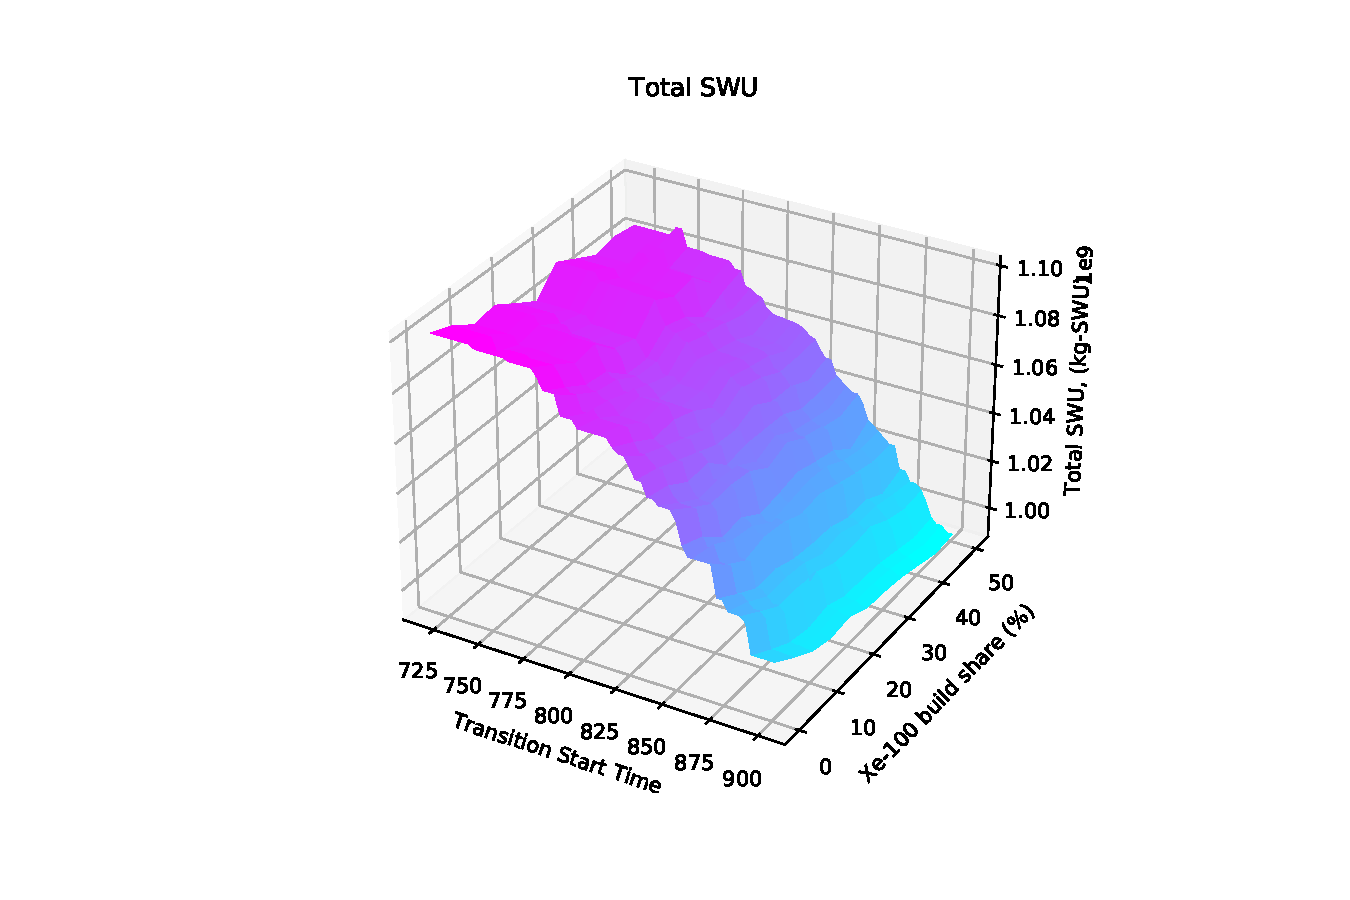
\includegraphics[scale=0.7, trim=120 0 120 0, clip]{ts_xe100_share_swu.pdf}
    \caption{Effect of transition start time and Xe-100 build share 
    on total fuel mass.}
    \label{fig:ts_xe100_share_swu}
\end{figure}

\subsection{Scenario 14}